\documentclass[12pt,oneside,english]{article}

\usepackage[T1]{fontenc}
\usepackage[latin1]{inputenc}
\usepackage{geometry}
\geometry{verbose,letterpaper,tmargin=1in,bmargin=1in,lmargin=1in,rmargin=1in}
\usepackage{textcomp}
\usepackage{babel}
\setcounter{secnumdepth}{0}
\usepackage{graphicx}
\usepackage{float}
\floatstyle{boxed}
\restylefloat{figure}
\usepackage{longtable}
\usepackage{url}

\newcommand{\BibTeX}{{\sc Bib}\TeX}


\begin{document}
\sffamily

        \title{in-situ impedance and morphology of self-assembling gold nanoislands}

	\author{John Donovan, Dr. Chuhee Kwon\\
	University of California, Long Beach, CA\\
	{\small donovan.csulb@gmail.com ckwon@csulb.edu}}
	
        \date{\today}

	\maketitle


        \section{Introduction}
	\subsection{background}
	Gold nanoislands  are formed by annealing a substrate -- on which gold has been uniformly deposited -- to produce islands within a predictable range of size and shape.
	The uniformity of the size and shape can be inferred by the width of the absorption features in the resulting thin film.
	\subsection{purpose}
	This research attempts to create reproducible samples of gold nano-islands and study their morphology.
	Prior research suggested that gold nano-island are sensitive to number of layers, method of depositing the gold, and variations in annealing temperature \cite{shon07}.
	Research on the self-assembly method used in this paper also depend on temperature profile of annealing and length of time (in days) between creation and annealing (\cite{joshi}).
	This research quantifies the repeatiblity of gold nano-islands produced using the label-free(*) self-assembly method.
	\subsection{method}
	Samples are produced using ***.

	\section{Procedure}

\begin{figure}
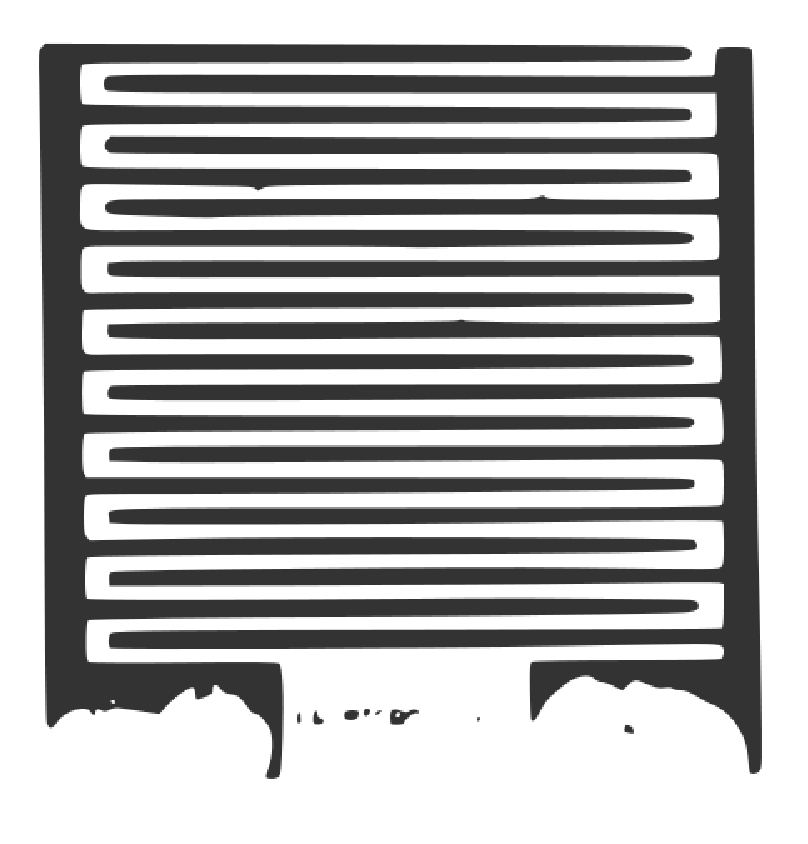
\includegraphics[scale=0.4]{images/IDE0.eps} \label{f:IDE}
\caption{The IDE}
\end{figure}
	


\clearpage
\bibliography{thesis_draft}
\bibliographystyle{plain}


\end{document}
%% The following is some template materials -- equations and figures.
\documentclass[aps,prl,twocolumn,oneside,showkeys,floatfix]{revtex4-1}
\newcommand{\BibTeX}{{\sc Bib}\TeX}
\usepackage{graphicx}
\usepackage{listings}

\newbox\bwk\edef\tempd#1pt{#1\string p\string t}\tempd\def\nbextr#1pt{#1}
\def\npts#1{\expandafter\nbextr\the#1\space}
\def\ttwplink#1#2{\special{ps:1 0 0 setrgbcolor}#2\special{ps:0 0 0 setrgbcolor}\setbox\bwk=\hbox{#2}\special{ps:( linkto #1)\space\npts{\wd\bwk} \npts{\dp\bwk} -\npts{\ht\bwk} true\space Cpos}}
        \begin{equation}
        \nu_{\mathtt{Larmor}} = {{\Delta E} \over{ 2 \pi \hbar}} = {{2 B \cdot \mu_{\mathtt{proton}}} \over{2 \pi \hbar}}
        \end{equation}

        \author{John \surname{Donovan}}
        \affiliation{CSULB}
        \begin{abstract}
                \begin{description}
                        \item[Background] This part would describe the
                        context needed to understand what the paper
                        is about.
                        \item[Purpose] This part would state the purpose
                        of the present paper.
                        \item[Method] This part describe the methods
                        used in the paper.
                        \item[Results] This part would summarize the
                        results.
                        \item[Conclusions] This part would state the
                        conclusions of the paper.
                \end{description}
        \end{abstract}
        \keywords{nano,nano-islands,thin films}
        \maketitle
        Written in \LaTeX\ with TexMaker.


\begin{figure}
\includegraphics[scale=0.5]{BField_Set1.eps} \label{BSet1}
\caption{The magnetic field (in MHz resonance frequency) measured.  Set 1 did not include many measurements of the most uniform part of the field.}
\end{figure}

\clearpage
\begin{widetext}
\section{Appendix}
\subsection{Spin Echo Peak-Finder Algorithm in Matlab}
\lstset{language=Matlab, basicstyle=\footnotesize, numbers=left, captionpos=t, breaklines=true, caption=find\_spin\_echo() locates the pulse maxima in a spin-echo pulse train, label=T2 Pulse Train, frame=shadowbox}
\lstset{basicstyle=\small\ttfamily, basewidth=0.51em}
\lstinputlisting{../find_pulse_train.m}
\end{widetext}


